\begin{frame}{MST Heuristik}
	\begin{itemize}
		\item MST Heuristik:
      \begin{itemize}
      	\item Länge durch MST Heuristik zwischen opimale Lösung und 2*optimale Lösung
      \end{itemize}
      \vspace{1cm}
      	\item Ablauf MST Heuristiken:
        \begin{enumerate}
        	\item minimum spanning tree mit Algorithmus von Kruskal erstellen 
            \item Kanten des minimum spanning tree verdoppeln
            \item Hierholzer Algorithmus
            \begin{itemize}
            \item einzelne Subtouren erstellen
            \item Eulertour bilden $\Rightarrow$ Subtouren zusammenfügen
            \end{itemize}
            \item Doppelte Punkte in Reihenfolge löschen
        \end{enumerate}
	\end{itemize}
\end{frame}

\begin{frame}{MST Heuristik}    
  \begin{columns}
	  \begin{column}{0.5\textwidth}
	\begin{itemize}
		\item Kruskalbaum und verdoppelte Kanten
      \vspace{1cm}
      	\item Hierholzer Algorithmus:
        \begin{enumerate}
        	\item einzelne Subtouren erstellen
            \item Eulertour bilden $\Rightarrow$ Subtouren zusammenfügen
        \end{enumerate}
        \item Doppelte Punkte in Reihenfolge löschen
        \item Endtour: 3-1-6-4-5-2-7-3
	\end{itemize}
	  \end{column}
      \begin{column}{0.5\textwidth}
      	\vspace{-1.0cm}
        \begin{figure} 
        	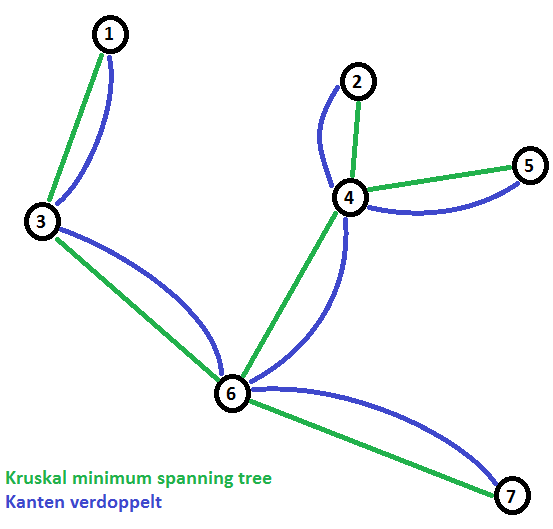
\includegraphics[scale=0.30]{Kruskal_double_edges.png} \\
            \vspace{.2cm}
            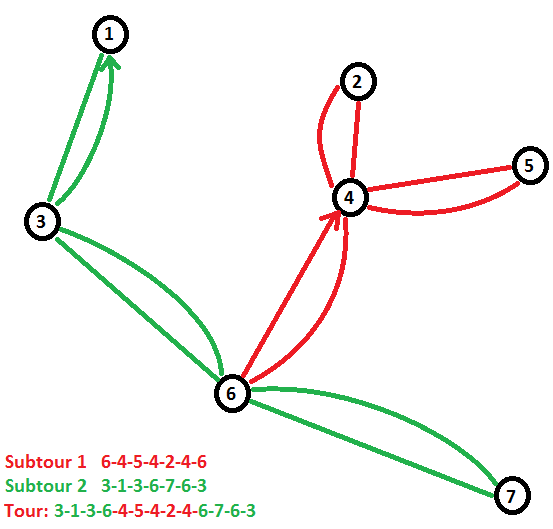
\includegraphics[scale=0.30]{Hierholzer.png}
        \end{figure}
  	  \end{column}
  \end{columns}
\end{frame}

\begin{frame}{Multi Fragment Heuristik}    
  \begin{columns}
	  \begin{column}{0.5\textwidth}
	\begin{itemize}
		\item Ablauf Multi Fragment Heuristik
            \begin{itemize}
        		\item kleinste Kanten zwischen zwei Punkten verbinden, ohne ein 						  Verzweigung zu erzeugen bis alle Punkten genau zwei Kanten besitzt
                \item führt zu einem Pfad, bis er am ende verbunden wird
                \item am anfang können mehrere kleine Pfade entstehen, die irgendwann 						miteinander verbunden werden
                \item Endtour: 2-4-5-7-6-3-1-2
            \end{itemize}
	\end{itemize}
	  \end{column}
      \begin{column}{0.5\textwidth}
      	\vspace{0.0cm}
        \begin{figure} 
        	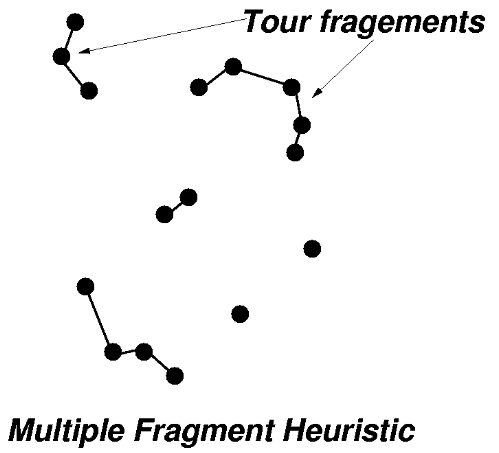
\includegraphics[scale=0.30]{Multi_fragment_2.png}\\
                  	\vspace{1.0cm}
            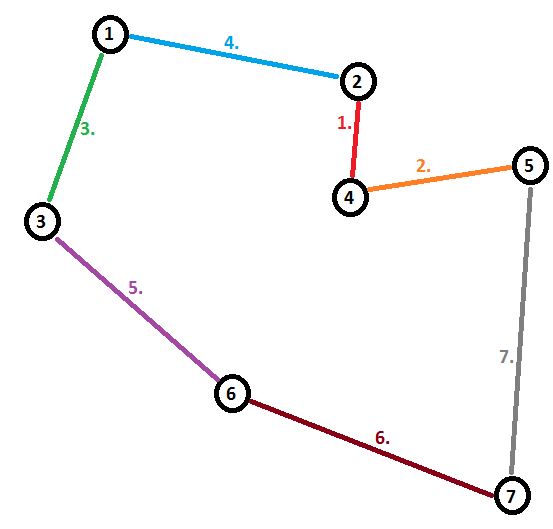
\includegraphics[scale=0.30]{Multi_fragment.png}
        \end{figure}
  	  \end{column}
  \end{columns}
\end{frame}